\vspace{-0.3cm}
\section{MATLAB Implementation and Results}\label{sec:matlab-results-slide-safety}
\vspace{-0.2cm}
The results shown in this section are based on the implemented controller found in \autoref{app:slide_implement_1} and in \autoref{app:cd} under the path \texttt{matlab\_scripts/slide\_controller/slide\_controller.m}. All plots are made with the following characteristics:
\vspace{-1mm}
\begin{itemize}
	\itemsep-0.7mm
\item The sampling rate is tested with both $f_s = 2\,$kHz (expected sampling rate in the long run) and $f_s = 100\,$Hz (current limitation of the sample rate caused by the TCP/IP communication channel).
\item The control signal is limited to $\pm 0.1$\,m (actual limit for slide movement).
\item The velocity is limited to $\pm$1\,m/s (conservatively estimated limit for slide movement).
\item The forward Euler method is used to extrapolate the states.
\item The design parameter $\kappa$ from \autoref{eq:control_law} is set to $\kappa=1$ (neutral).
\item The simulation time is 5\,s. Various setpoints ought to indicate the behaviour in different regions.
\end{itemize}
The \texttt{model} variable in the first line in \autoref{app:slide_implement_1} is set to the number 1 for the first order model and 2 for the second order model. 


\subsection{MATLAB Results based on First Order Model}\label{subsec:matlab-results-1order}
\vspace{-1mm}
The state trajectory composing slide position is plotted in \autoref{fig:trajectory1},
%\vspace{-3mm}
\begin{figure}[htbp]
\hspace*{-5mm}\vspace*{-1mm}
\subbottom[State trajectory with $f_s = 2\text{kHz}$.]{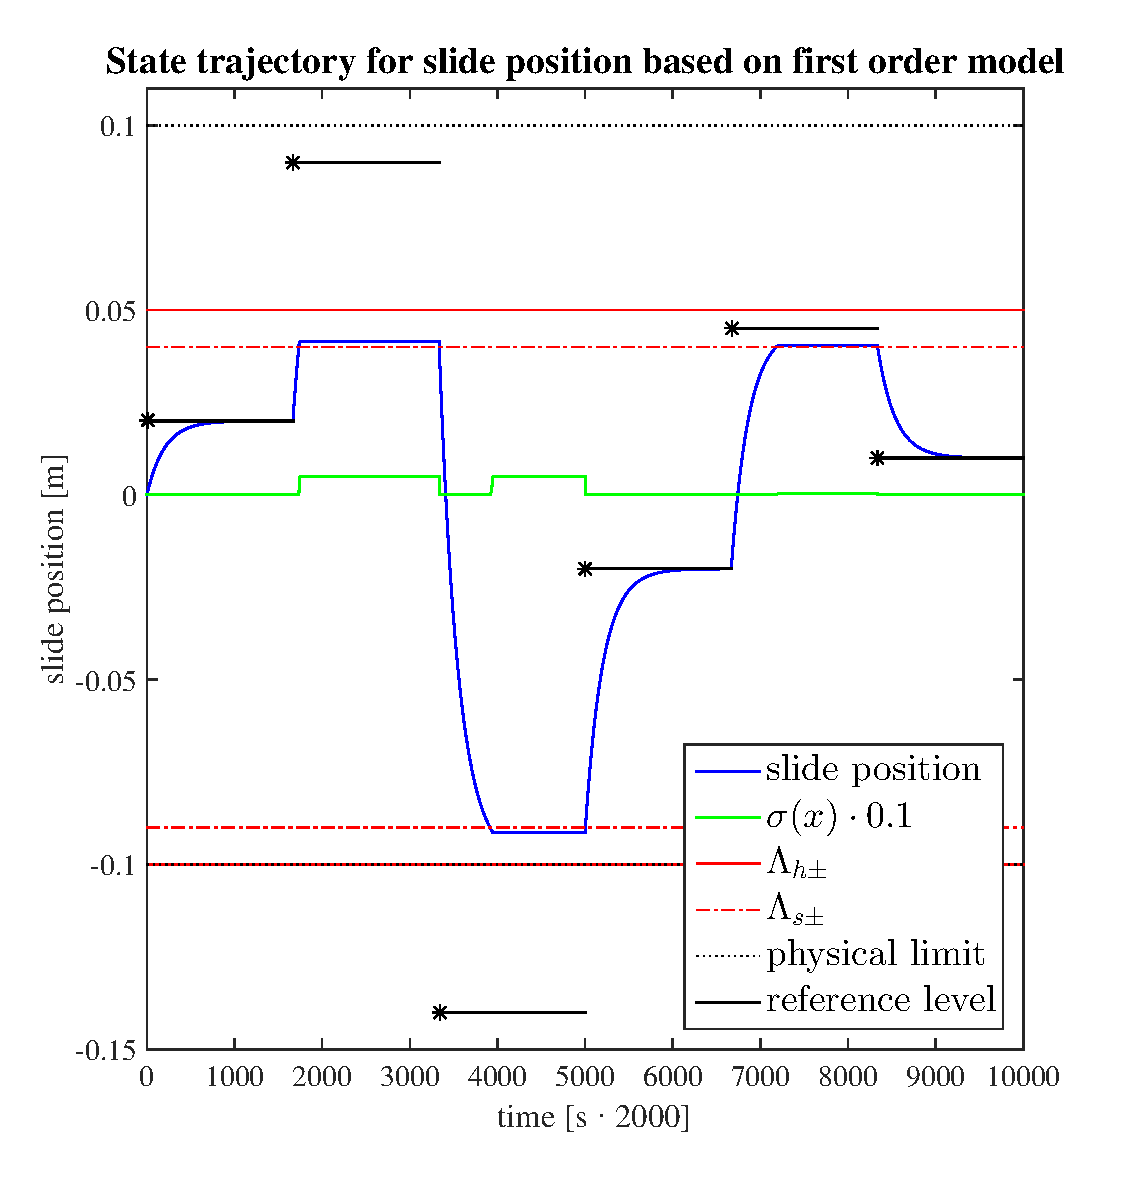
\includegraphics[width=0.55\textwidth]{trajectory_2kHz.pdf}\label{fig:2khz_1}}%
\subbottom[State trajectory with $f_s = 100\text{Hz}$.]{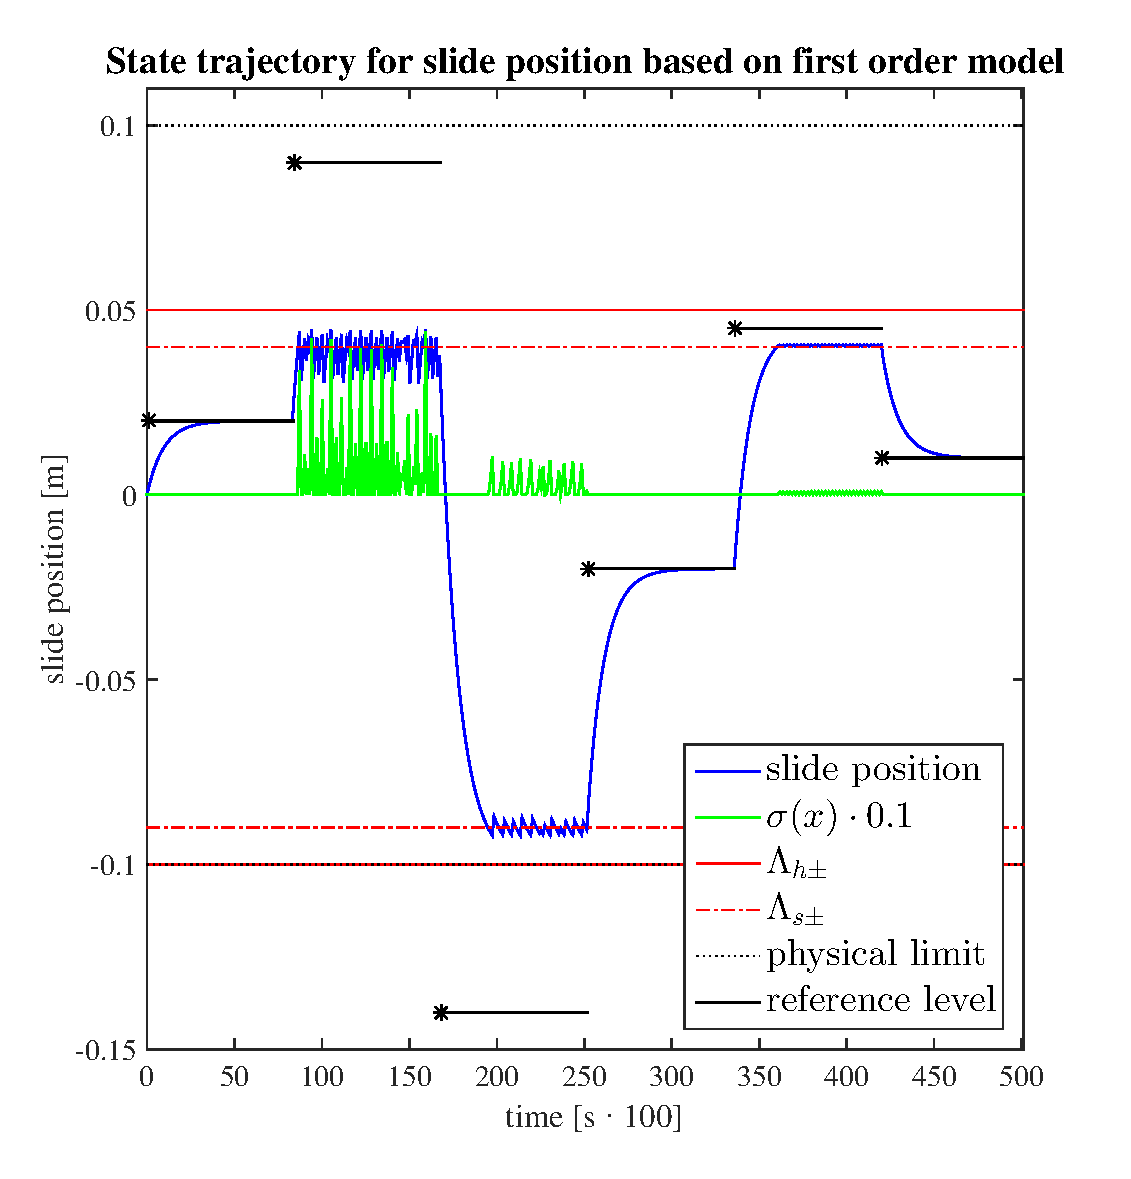
\includegraphics[width=0.55\textwidth]{trajectory_100Hz.pdf}\label{fig:100hz_1}}%
\caption{State trajectory for slide position for $\kappa=1$. The MATLAB implementation can be found in \autoref{app:slide_implement_1}. The plot is based on forward Euler.}
\label{fig:trajectory1}
\end{figure}
%
%
%\begin{figure}[H]
%	\center
%		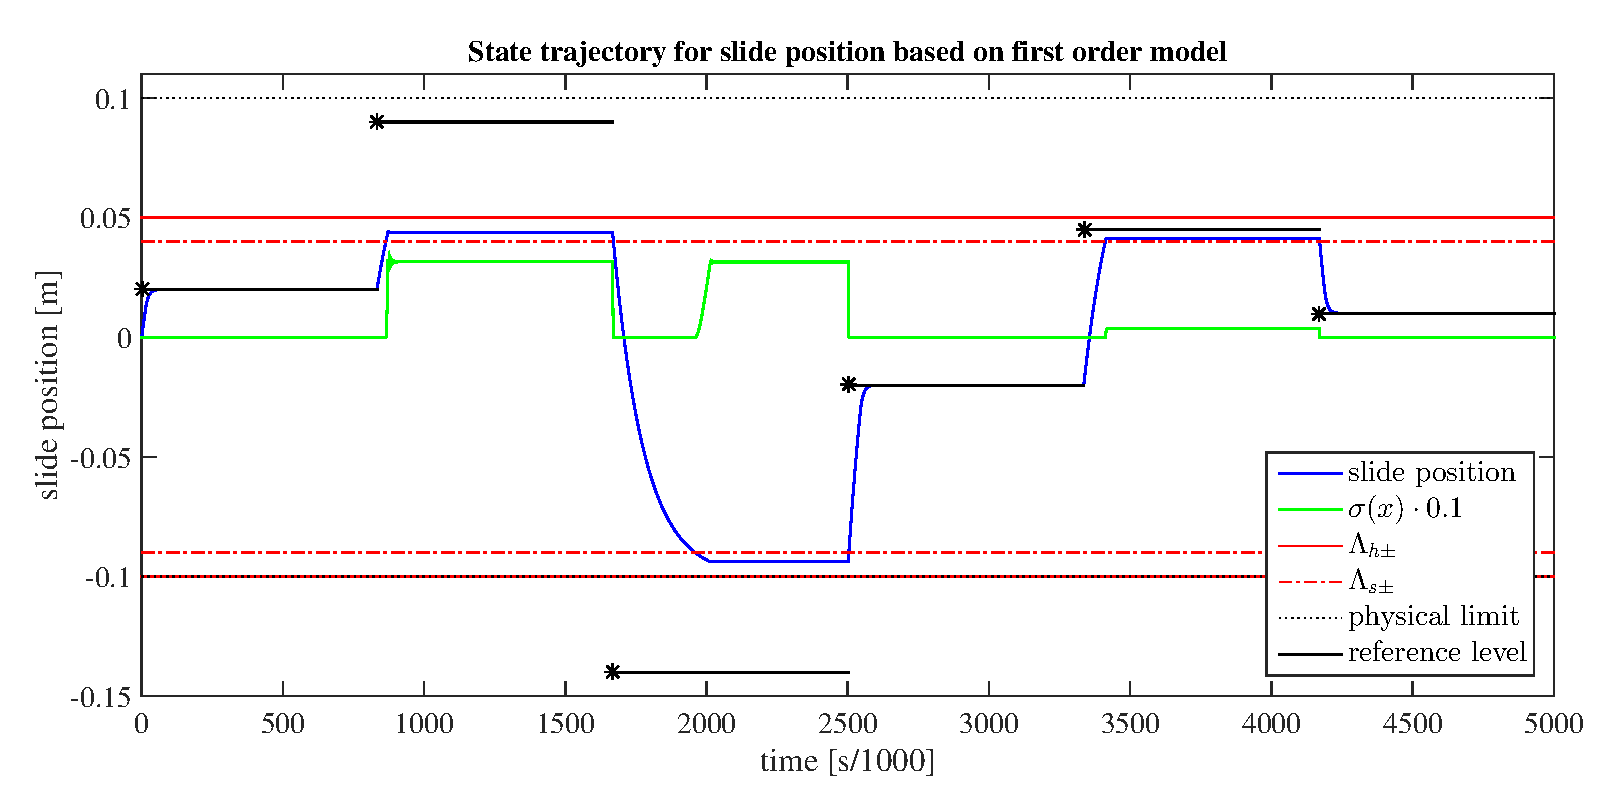
\includegraphics[scale=0.6]{trajectory_slide.eps}
%	\caption{State trajectory for slide position for $\kappa=1$. MATLAB implementation can be found in \autoref{app:slide_implement_1}. The plot is based on forward euler with a sampling rate of $1\,$kHz. It is seen how the correct position is obtained in the interval $[\Lambda_{s-}:\Lambda_{s+}$]. When setpoints are given outside the safe area, the safety controller ensures that the hard boundaries $\Lambda_{h+}$ and $\Lambda_{h-}$ are not exceeded at any time and that the position finds its equilibrium at some arbitrary state.}
%	\label{fig:trajectory1}
%\end{figure}
%\vspace{-2mm}
from which it is seen how the correct position is obtained in the interval $[\Lambda_{s-},\Lambda_{s+}$]. When setpoints are given outside the safe area, the safety controller ensures that the hard boundaries $\Lambda_{h+}$ and $\Lambda_{h-}$ are not exceeded at any time and that the position finds its equilibrium at a state determined by the linear combination of the two controllers. It is, however, noted that lowering the sampling frequency to 100\,Hz entails a closed loop system which is too fast compared to the sampling rate, and for setpoints outside the safe region, the position is oscillating between linear and safety control.

To verify that \autoref{req2} is fulfilled in the simulation, the Lie derivatives are plotted in \autoref{fig:lie1}, from which it can be seen that $L_gB(x) \neq 0 \,\, \forall x \neq \frac{-b}{2a}$, and that $L_fB(x)=0$ in $x = \frac{-b}{2a}$, which essentially fulfils \autoref{req2}. Indeed, even for $\mathcal{X}$ defined as the entire range $[\Lambda_{h-},\Lambda_{h+}]$ (compare to \autoref{tab:intervals}), the chosen CBF would have been valid because the only place where $L_gB(x) = 0$ is at the critical point. Note also that the Lie derivatives are independent of the scalar $\kappa$.
%\vspace{-2mm}
\begin{figure}[H]
\hspace{-7mm}
		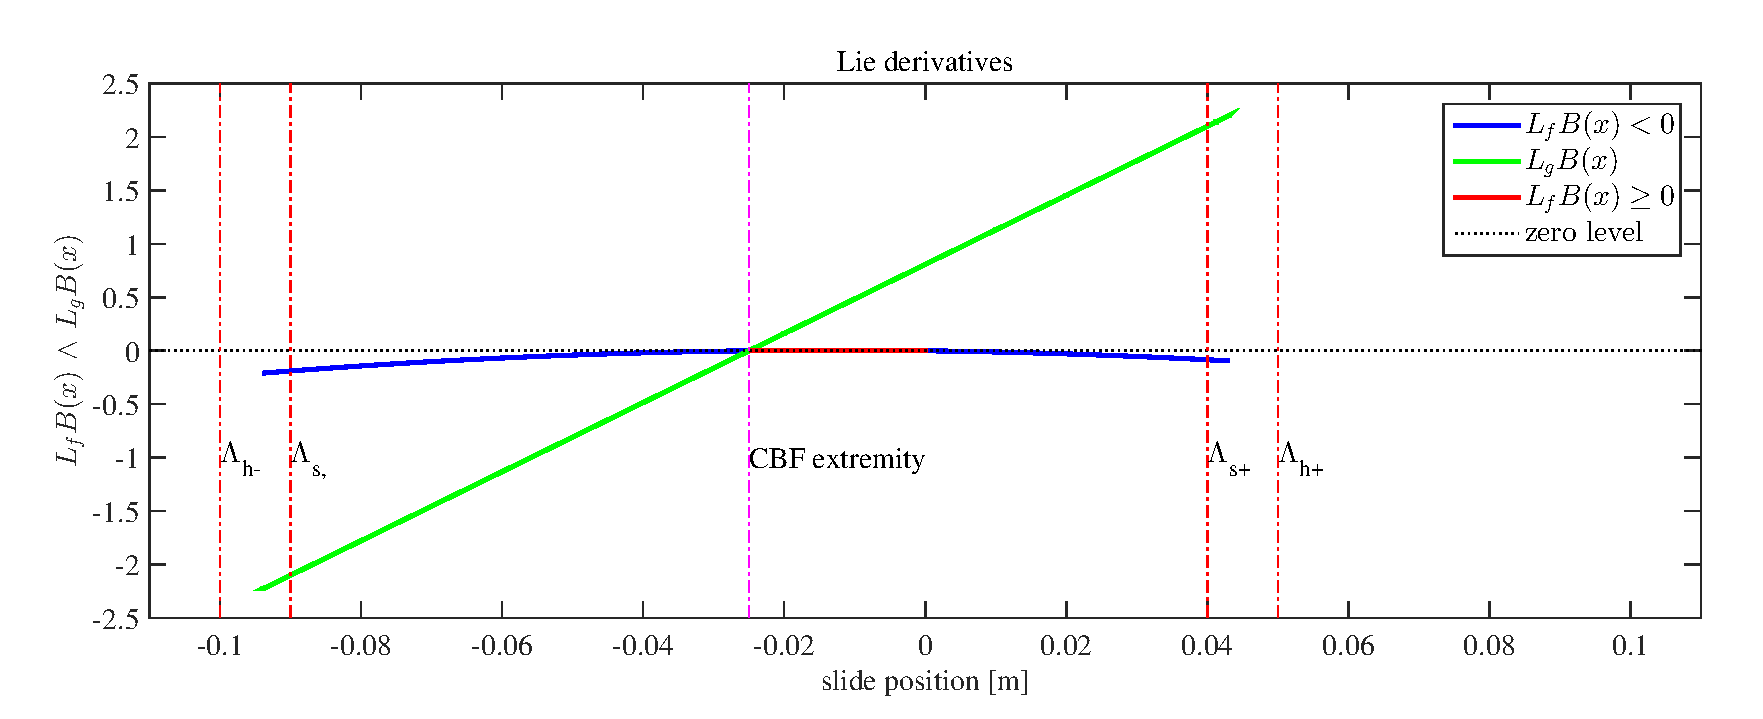
\includegraphics[width=1.1\textwidth]{Lie_slide_1d.eps}
	\caption{Lie derivatives of the CBF along the vector fields $f(\mathbf{x}) = \textbf{Ax}$ and $g(\mathbf{x})=\mathbf{B}$. %It is seen that $L_gB(x) \neq 0 \,\, \forall x \neq \frac{-b}{2a}$, and that $L_fB(\mathbf{x})=0$ in $x = \frac{-b}{2a}$ which essentially fulfils \autoref{req2}.
		}
	\label{fig:lie1}
\end{figure}
%For the record, the control signal is plotted in \autoref{fig:control1}.
%\begin{figure}[H]
%	\center
%		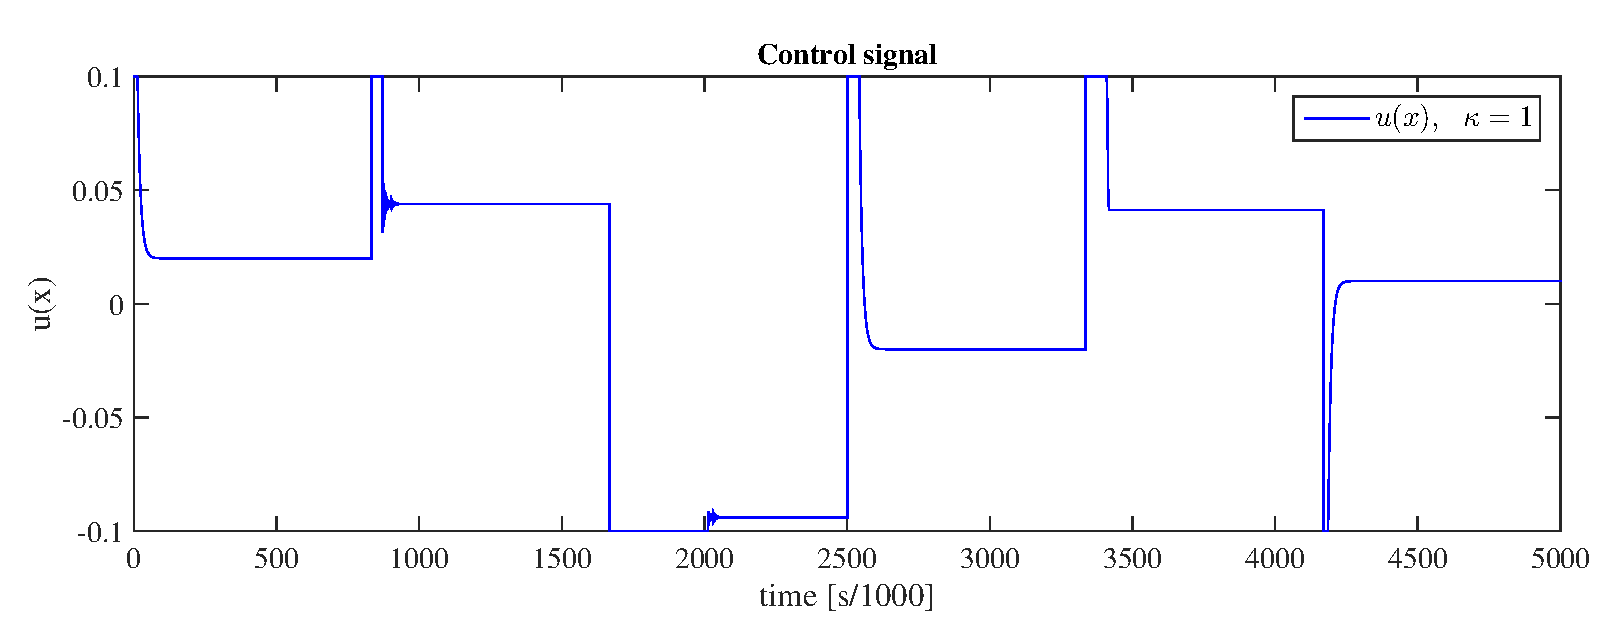
\includegraphics[scale=0.55]{control_slide_1.eps}
%	\caption{Control signal for $\kappa=1$. It is seen how the controller counteracts the large difference in setpoints given and in that way ensures safety. It is seen that when the absolute value of the setpoints are increased then $u(x)$ increases accordingly. The plot is ideal as no saturation constraints are given.}
%	\label{fig:control1}
%\end{figure}
%It is seen from \autoref{fig:control1} how the control signal reacts instantaneously and quite aggressive when $\Lambda_s$ is exceeded to counteract the large difference in setpoints given. It is also noted how the controller eventually settles smootly even when setpoints are given in the interval $[-\infty:\Lambda_{s-}]$ and $[\Lambda_{s+}:\infty]$. However, as the setpoints approaches $\pm \infty$, the sampling rate must also converge towards infinity. This is obviously not a realistic scenario as the slide movement is physically constrained.

Varying $\kappa$ increases the aggressivity of the safety controller and can create fluctuations in the transition area if the sampling rate is too low. Likewise $\sigma(x)$ will fluctuate along with an increased $\kappa$. One must be careful when increasing $\kappa$ when the sampling rate is relatively low. %The effect of increasing $\kappa$ ten times is shown in \autoref{fig:trajectory2}.
%\begin{figure}[H]
%	\center
%		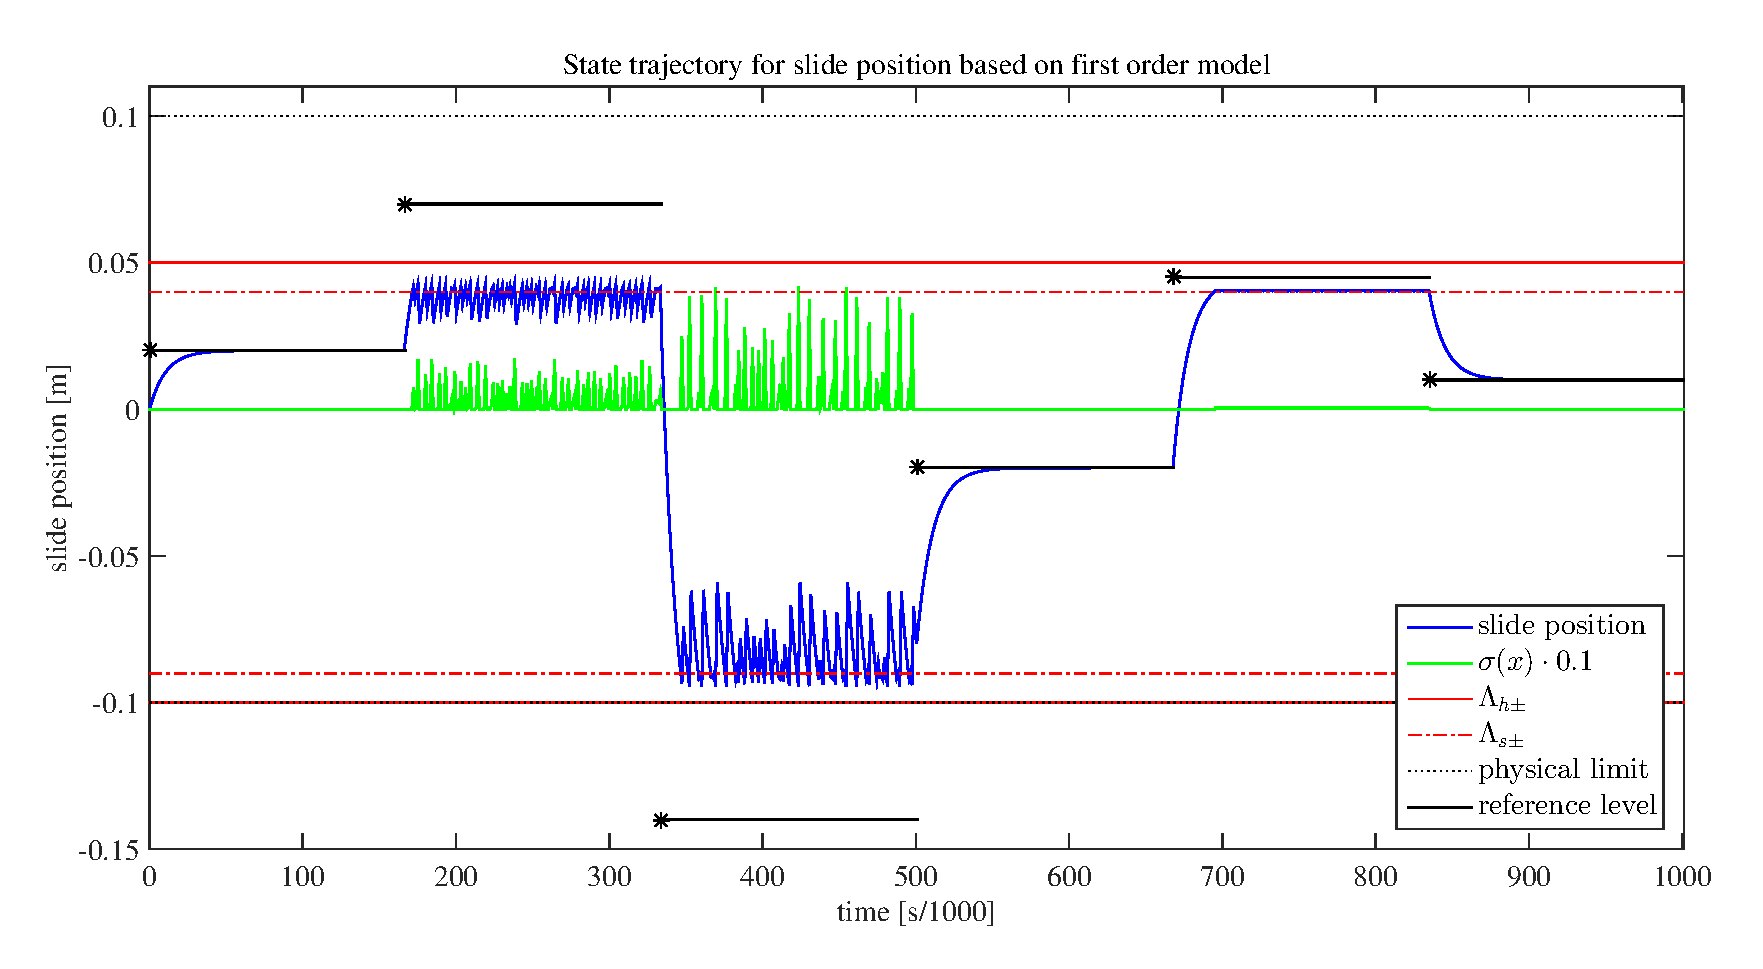
\includegraphics[scale=0.5]{trajectory_slide_kappa_10.eps}
%	\caption{State trajectory for slide position for $\kappa=10$ based on same control law and model as \autoref{fig:trajectory1}. It is seen how the safety controller is more aggressive.}
%	\label{fig:trajectory2}
%\end{figure}


%\vspace{-0.3cm}
\subsection{MATLAB Results based on Second Order Model}\label{subsec:matlab-resutls-2-order}
\vspace{-0.2cm}
The state trajectory composing slide position based on the second order model is shown in \autoref{fig:traject2}.
It is seen how the boundaries are respected at all time regardless of irresponsible setpoints within the unsafe region, which cause $\sigma(\mathbf{x})$ to increase and thereby letting the control law be the linear combination of the safety controller $u(\mathbf{x}) = k_0(\mathbf{x})$ and the linear controller by pole-placement $\tilde{u}(\mathbf{x})$.
The state trajectory shown in \autoref{fig:traject2} verifies that the slide position does not exceed its limits even when setpoints are given outside the safe region.
\vspace{-2mm}
\begin{figure}[H]
\hspace*{-5mm}\vspace*{-1mm}
\subbottom[State trajectory with $f_s = 2\text{kHz}$.]{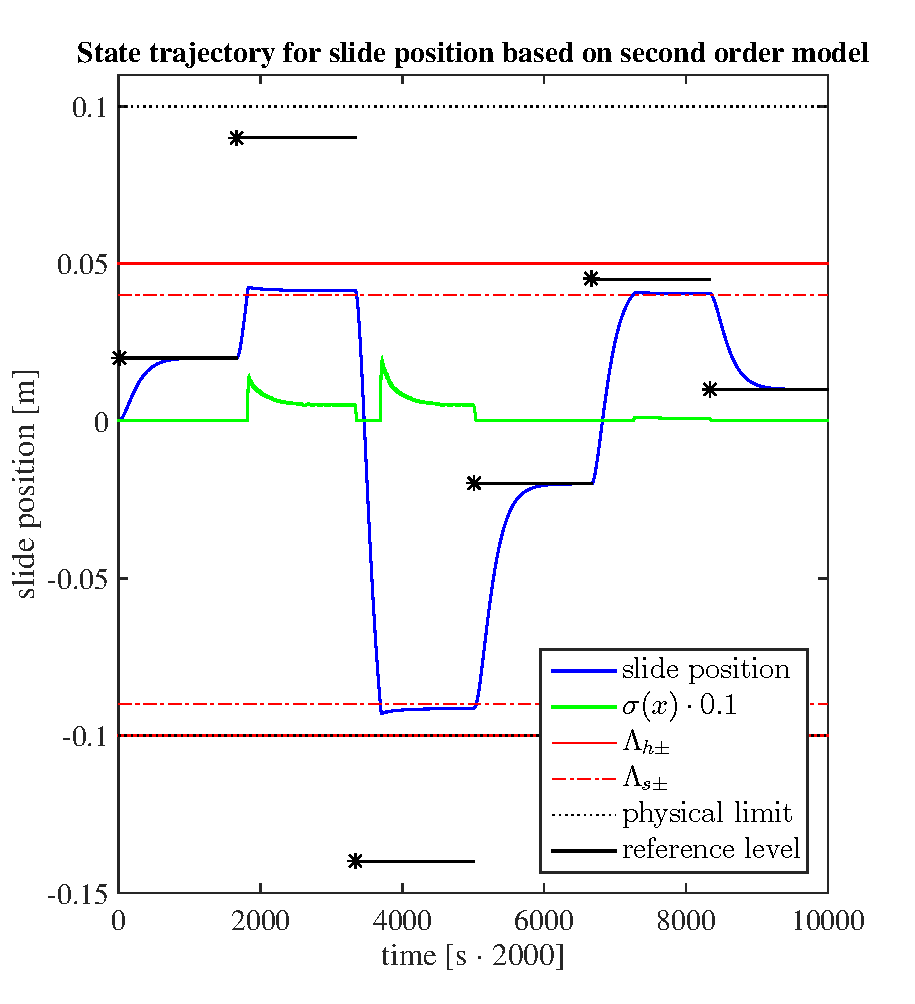
\includegraphics[width=0.55\textwidth]{trajectory_2_2kHz.pdf}\label{fig:2khz_2}}%
\subbottom[State trajectory with $f_s = 100\text{Hz}$.]{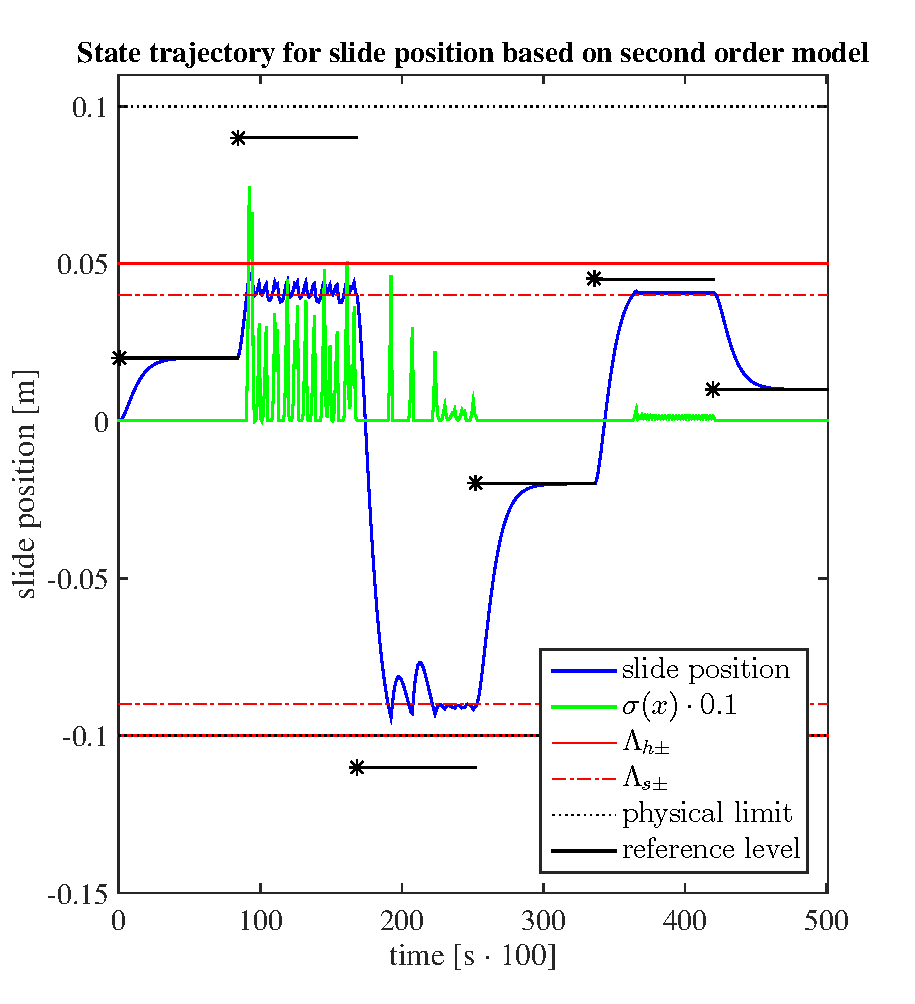
\includegraphics[width=0.55\textwidth]{trajectory_2_100Hz.pdf}\label{fig:100hz_2}}%
\caption{State trajectory for position based on second order system approximation.}
\label{fig:traject2}
\end{figure}
%
%
%
%
%\begin{figure}[H]
%	\center
%		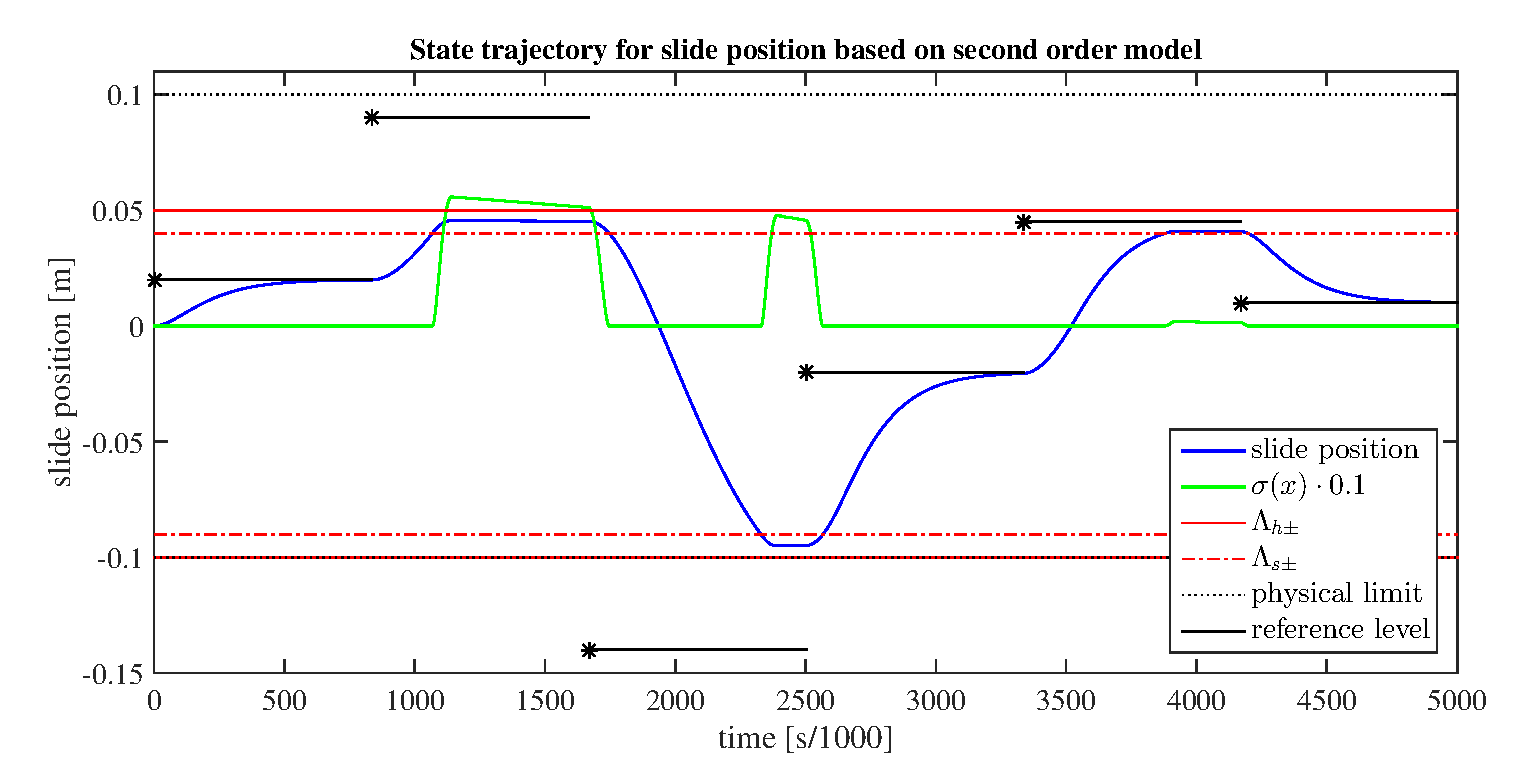
\includegraphics[scale=0.6]{trajectory_slide_second_order_model_kappa_1.eps}
%	\caption{State trajectory for position based on second order system approximation. It is seen how the boundaries are respected at all time regardless of irresponsible/unsafe setpoints. It is seen how $\sigma(x)$ 	increases when setpoints are given in the unsafe area. AS a result, the control law is a linear combination of the safety controller $u(x) = k_0(x)$ and the linear controller by pole-placement $\tilde{u}(x)$.}
%	\label{fig:traject2}
%\end{figure}


The Lie derivatives for the second order model and CBF are plotted in \autoref{fig:lie2}.
It is seen how $L_gB(\mathbf{x}) = 0$ and $L_fB(\mathbf{x}) = 0$ at the same time which in general is critical but accepted in this specific case as it is caused by $x_2=0$ which implies $u(\mathbf{x})=0 \,\,\, \Rightarrow \,\,\, x_1 \rightarrow 0$ which is safe.
\begin{figure}[H]
\hspace{-7mm}
		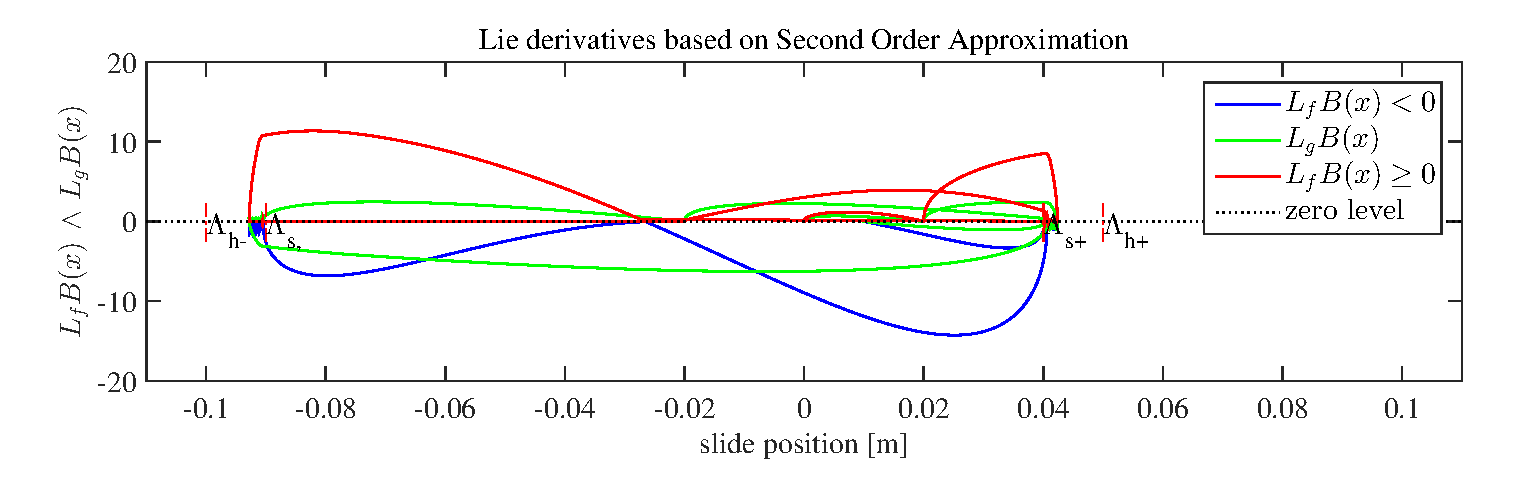
\includegraphics[width=1.1\textwidth]{Lie_slide_2d.eps}
	\caption{Lie derivatives of the CBF for the second order model. }
	\label{fig:lie2}
\end{figure}
%The constrained control signal is plotted in \autoref{fig:control2}
%\begin{figure}[H]
%	\center
%		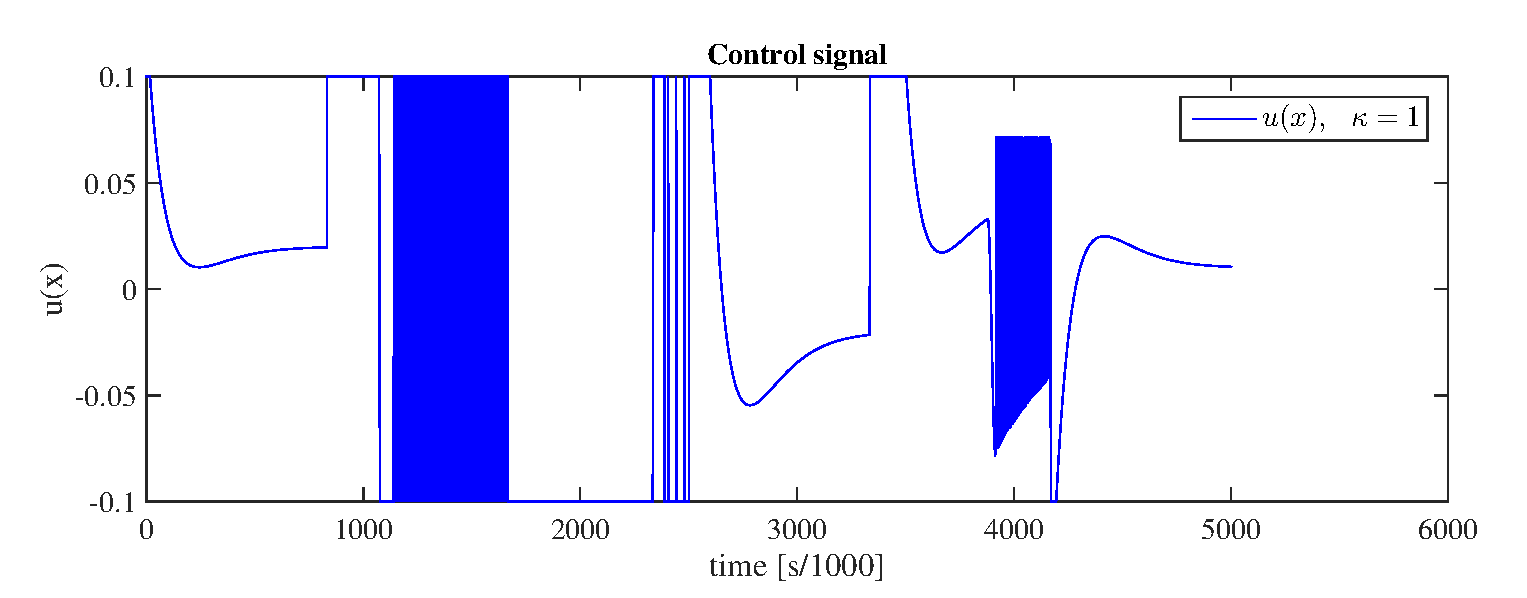
\includegraphics[scale=0.5]{control_signal_2.eps}
%	\caption{Control signal. It is seen how the it fluctuates heavily when $x_1 \in \Delta_t$ due to the position gradient.}
%	\label{fig:control2}
%\end{figure}
%It is from \autoref{fig:control2} noted how the control signal fluctuates heavily. This is because the position gradient (the velocity) changes sign constantly in the unsafe region as the trajectory seeks to go either one or the other way due to the safety controller and the setpoint given outside the safe region.
\subsection{Observer Verification}
The observer developed in \autoref{sec:K_Nbar_1D_2ndorder} will be verified with a step input at 1\,cm. The estimated position and velocity is plotted with the success criteria that $\hat{x}_1 = x_\text{ref}$ for $t \rightarrow \infty$ and that no overshoot in the position occurs. The velocity must stay within a reasonable velocity span, i.e. below 1\,m/s when the time constant is considered. The error is defined as $\hat{y}$--$y$ and must obviously stay very low in steady state.

The result is plotted in \autoref{fig:observerplot} from which it is seen how the position, velocity and error all complies with the expected outcome and fulfil the requirements.
\begin{figure}[H]
\hspace{-7mm}
		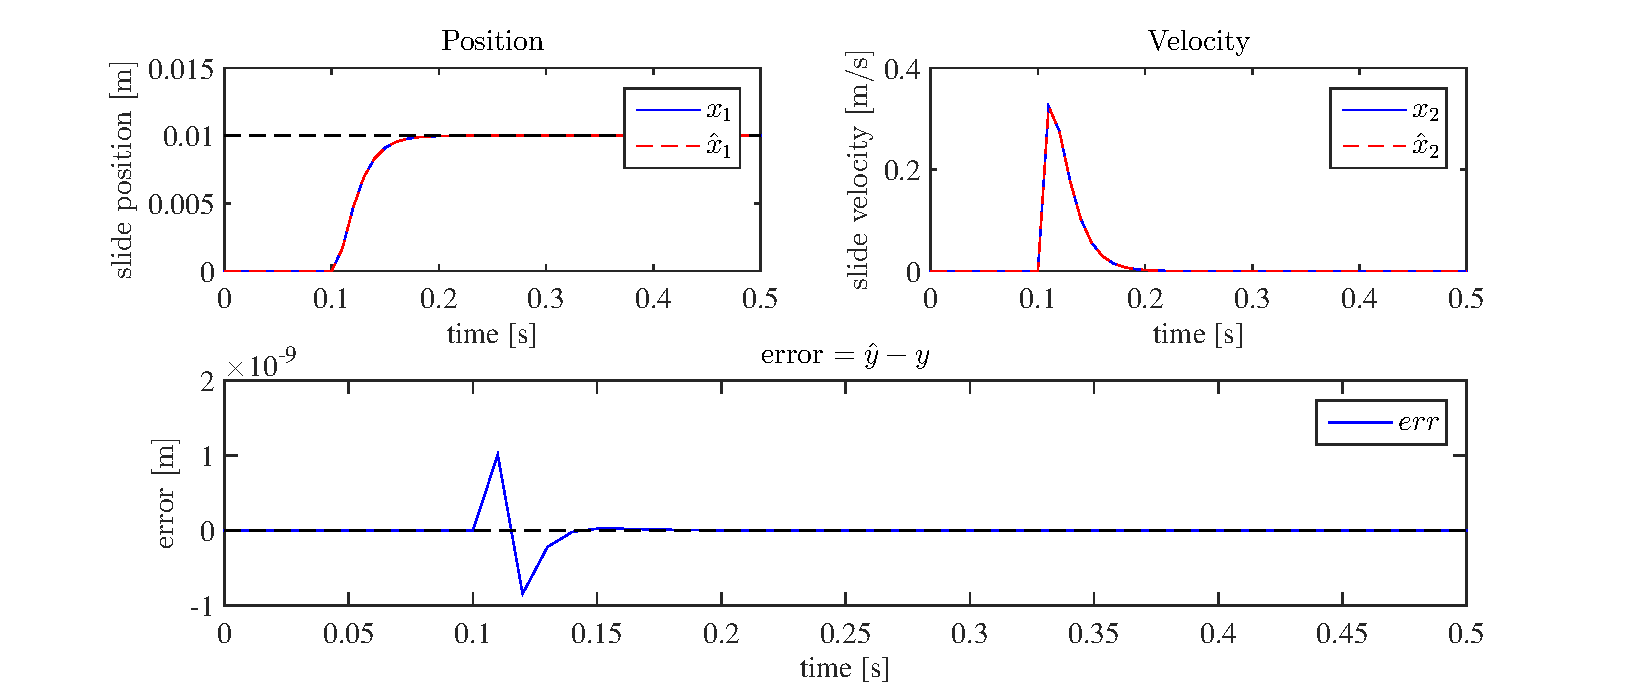
\includegraphics[width=1.1\textwidth]{observer_plot.eps}
	\caption{Simulation results from the simulink implementation of the observer. Plot details and simulink file can be found in \autoref{app:cd} by running \texttt{run\_observer.m} under the path \texttt{matlab\_scripts/observer/}.}
	\label{fig:observerplot}
\end{figure}
The outlined plots throughout this section concludes the MATLAB simulation. The MATLAB implementation shows the expected scenario, i.e. that the state trajectory complies with the outlined safe and unsafe regions. It shall now be seen how to implement the results on the Da Vinci robot itself.

\section{Implementation on the Da Vinci Robot}\label{sec:davinci-implementation}
The implementation constitutes the below listed bullet points:
\vspace{-2mm}
\begin{itemize}
	\itemsep-1mm
\item The controller will be implemented in C++. \textbf{Reason:} Along with Python, C++ is \underline{the} ROS compatible standard. The reason to use C++ over Python is to optimize speed performance. Furthermore, it is the general opinion among ROS experts (such as Postdoc Karl Damkj\ae r Hansen and others) that C++ is more useful in robot simulations and development and lastly, the already existing code at the Robotic Surgery Group - Aalborg University, is by far mostly developed in C++. However, Python as a scripting language, may be more user friendly, easier to get started with and in many cases more readable.
\item Real-time signal processing to ensure fixed sample rates. \textbf{Reason:} The observer matrices are built upon fixed sampling rates and for that reason it is crucial to comply with a fixed sample rate.
\item Algorithm development to connect these two bullet points.
\end{itemize}

\begin{figure}[H]
	\center
		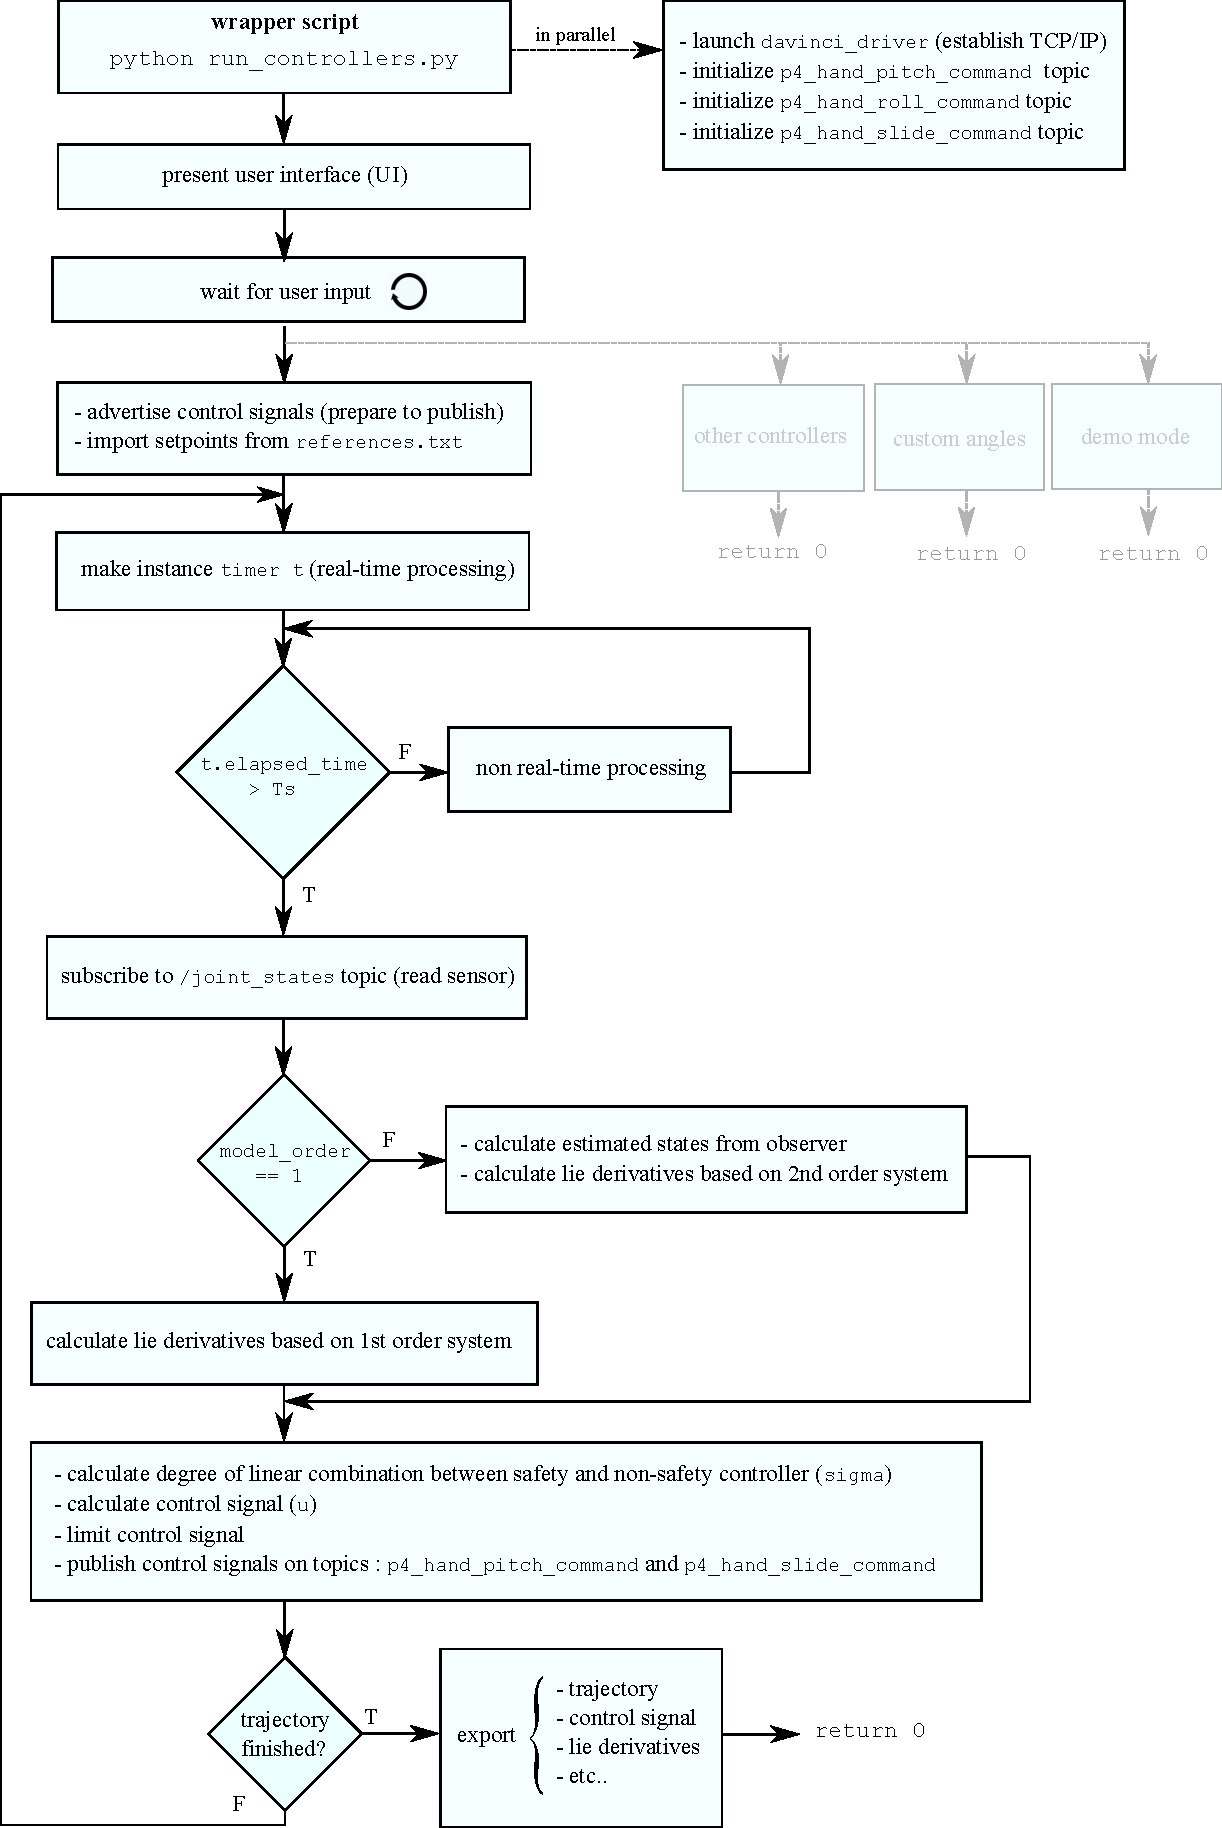
\includegraphics[scale=0.7]{flowchart_safety_controller.pdf}
		\vspace{2mm}
	\caption{Algorithm for slide safety controller. The source code associated with the algorithm can be found in \autoref{app:slide_implement_2} and in \autoref{app:cd}. It can also be found at github at the Robotic Surgery Group - Aalborg University under the repository \texttt{gr1032} (\textit{https://github.com/AalborgUniversity-RoboticSurgeryGroup/}).}
	\label{fig:slide_safery_algorithm}
\end{figure}
The controller is implemented at the highest abstraction layer, i.e. the ROS environment depicted in \autoref{fig:overview}. While ROS runs on most Linux laptops, it is not ROS itself that puts forth limitations for real time signal processing, neither is it the potentiometers that measures the angle. The bottleneck is caused by the TCP/IP communication channel which according to Assistant Engineer Simon Jensen is limited to 100\,Hz. For that reason, the maximum allowed execution time $c_{p,\text{max}}$ is:
\begin{flalign*}
	c_{p,\text{max}} = \dfrac{1}{100\,\text{Hz}} = 10\,\text{ms}
\end{flalign*}
The main algorithm is depicted in \autoref{fig:slide_safery_algorithm}, and the source code
can be found in \autoref{app:slide_implement_2} and in \autoref{app:cd}.

\subsection{Implementation on the Da Vinci Robot based on First Order Model}\label{subsec:implement-davinci-1d}
All plots and measurements in this subsection can be reconstructed by running the MATLAB script \texttt{plot\_data} found in \autoref{app:cd} in the folder \texttt{measurements/slide\_safety\_controller/1D\_1st\_order}. The execution time is validated first as it is essential for the controller to complete successfully. \Autoref{fig:exe_1} shows a plot of measured execution time for each iteration, verifying that $c_p < c_{p,\text{max}}$ and thereby the real-time part.
\begin{figure}[H]
	\center
		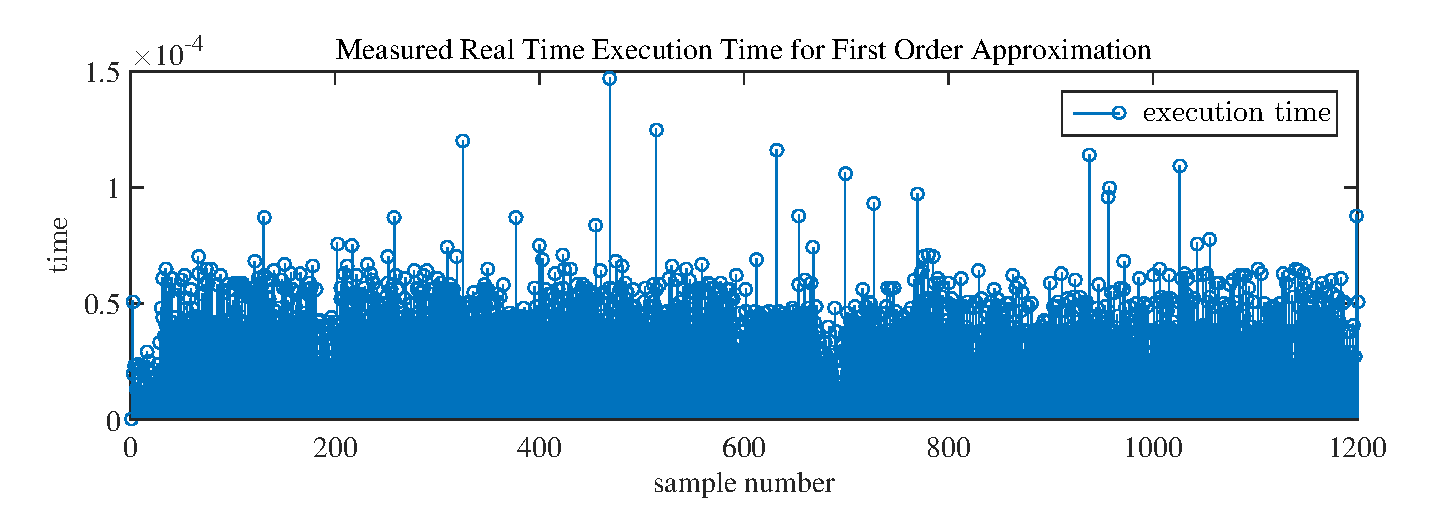
\includegraphics[scale=0.6]{execution_time_1_order.eps}
	\caption{Execution time for the first order system approximation. It is seen that the controller never exceeds a computation time of 150\,$\mu$s.}
	\label{fig:exe_1}
\end{figure}



%\vspace{-10mm}
\begin{figure}[htbp]
\hspace{-7mm}
		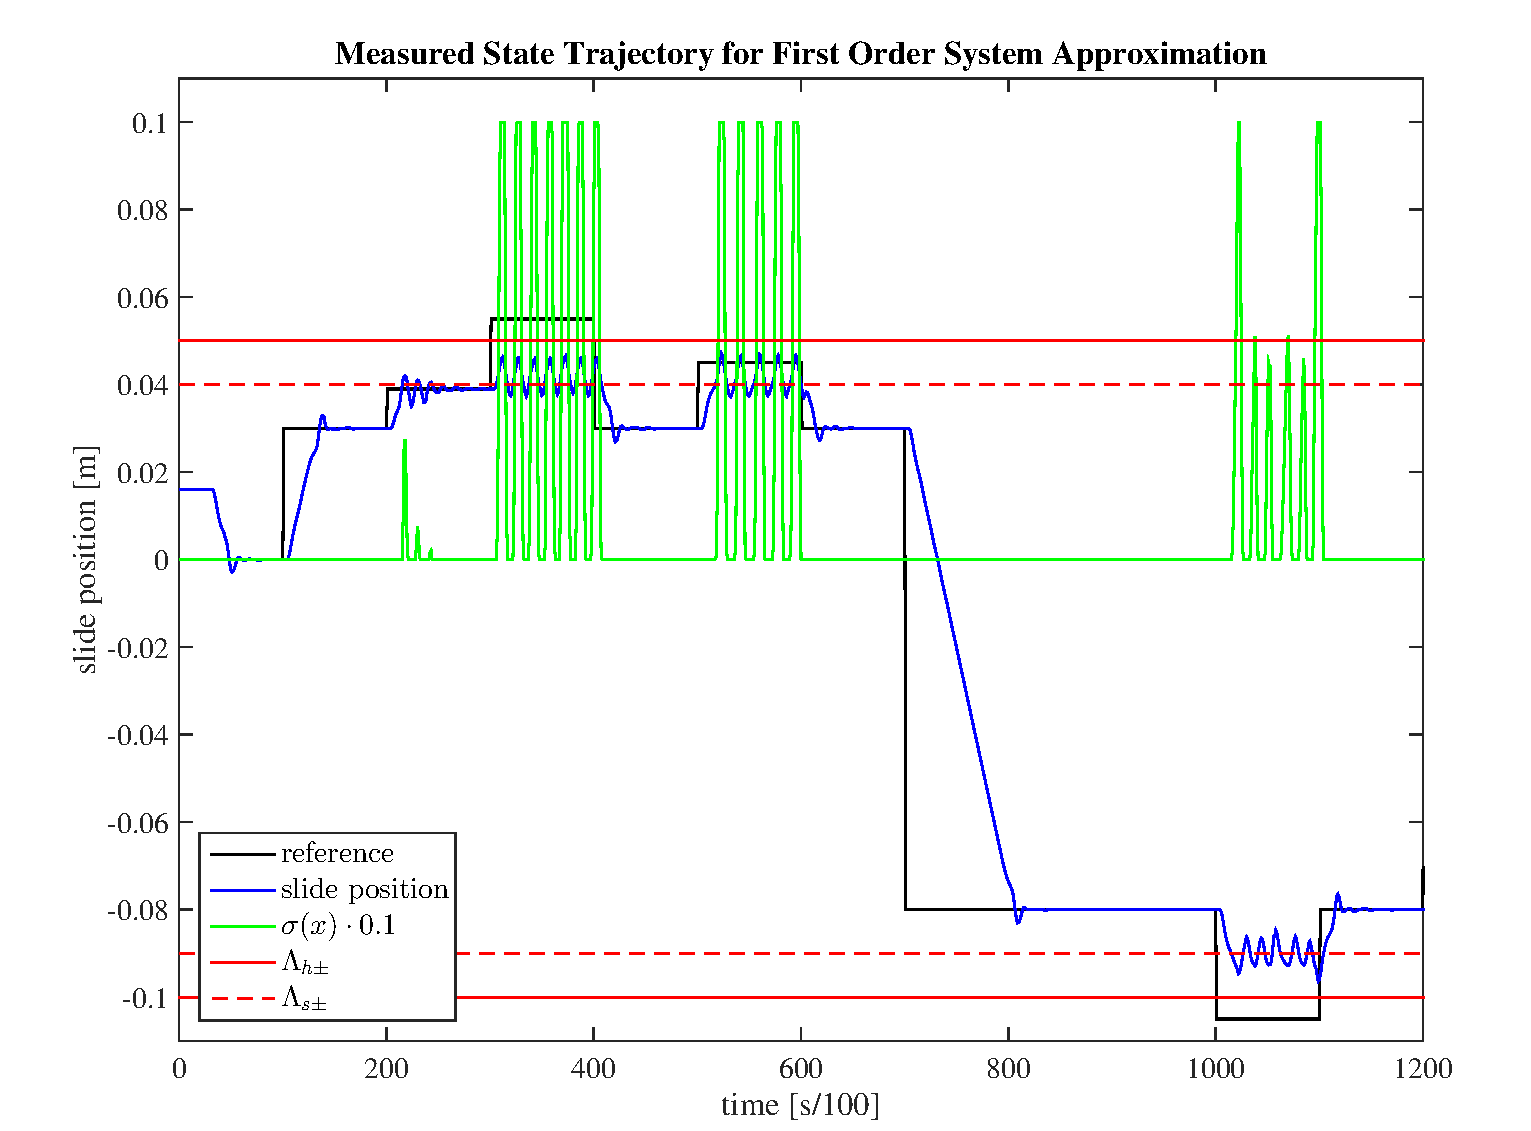
\includegraphics[width=1.1\textwidth]{trajectory_slide_meas_1.eps}
	\caption{Measured position trajectory based on the first order system approximation.}
    \label{fig:traj_meas_1}
\end{figure}
The measured state trajectory is plotted in \autoref{fig:traj_meas_1}.
Here it is seen how the controller ensures that $x \in \mathcal{X}_u^c \ \ \forall \, x$. The poor system approximation is also revealed as the trajectory has an overshoot which was not included in the simulation found in \autoref{fig:trajectory1}. This is however not surprising as the first order approximation was created to simplify the control barrier function and to avoid the observer design as an initial approach. A consequence of the overshoot is seen when setpoints very close to $\Lambda_{s+}$ are given. The slide movement starts to oscillate which is caused by $\sigma(x)$. This is obviously not a good thing, but nevertheless it is the intended outcome when $x \in \mathcal{T}$. Additionally, it is seen how $\sigma(x)$ allows $k_0(x)$ to force the position from reaching its setpoint when $x_\text{ref} \in \mathcal{X}_u$ but allows $x$ to cross $x_\text{ref}$ when $x_\text{ref} \in \mathcal{T}$. %This is indeed the effect of $\sigma(x)$. 
It is finally seen that the safety controller is fully functional for both $\mathbb{R}^-$ and $\mathbb{R}^+$.

The Lie derivatives are calculated based on the measured position. The result is seen in \autoref{fig:meas_lie_1}.
It is seen that the Lie derivatives from \autoref{fig:meas_lie_1} are very similar to the theoretical Lie derivatives from \autoref{fig:lie1}.

%\vspace{-10mm}
\begin{figure}[htbp]
\hspace{-3mm}
		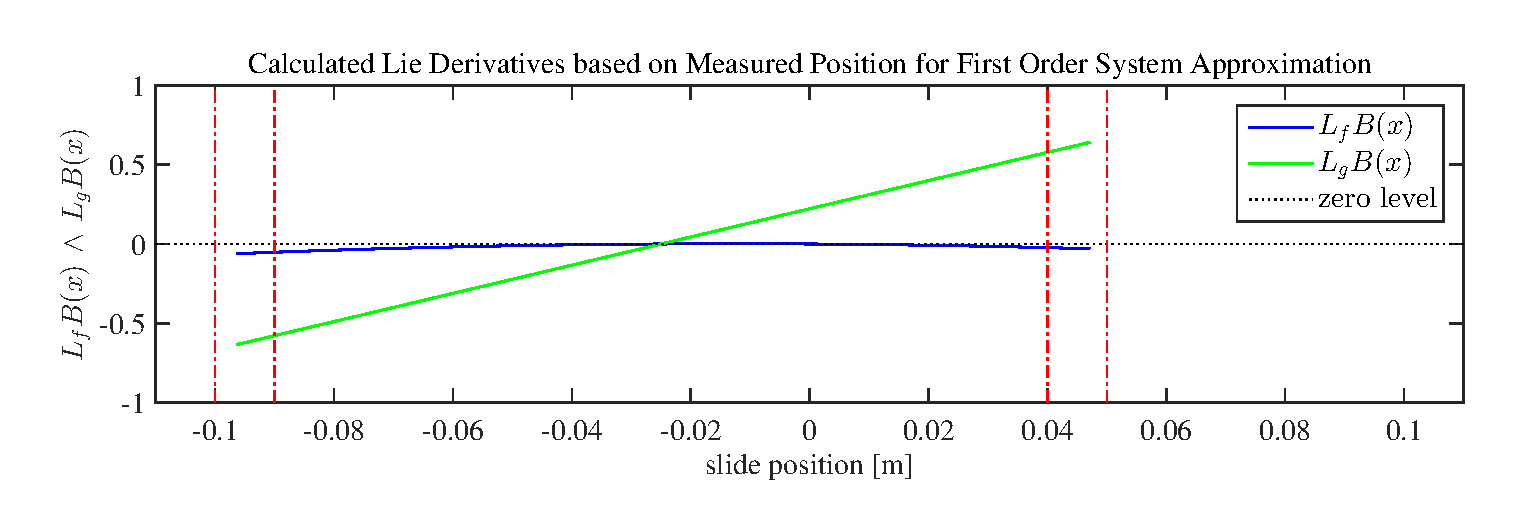
\includegraphics[width=1.05\textwidth]{meas_lie_1.eps}
	\caption{Calculated Lie derivatives based on measured position for the first order approximation. }
    \label{fig:meas_lie_1}
\end{figure}

%%%%%%%%%%%%
%%%%%%%%%%%%
%%%%%%%%%%%%
%%%%%%%%%%%%

\subsection{Implementation on the Da Vinci Robot based on Second Order Model}\label{subsec-implement-2dmodel}
\vspace{-1mm}
All plots and measurement in this subsection can be reconstructed by running the MATLAB script \texttt{plot\_data} found in \autoref{app:cd} in the folder \texttt{measurements/slide\_safety\_controller/2D\_2nd\_order}. Again, the execution time is validated first. A plot of measured execution time for each iteration is shown in \autoref{fig:exe_2}.
It is seen that the real time part is completed within the allowed 10\,ms (100\,Hz). Note that the execution time is slightly higher than in \autoref{fig:exe_1} because the velocity is estimated with the observer.


\begin{figure}[htbp]
	\center
		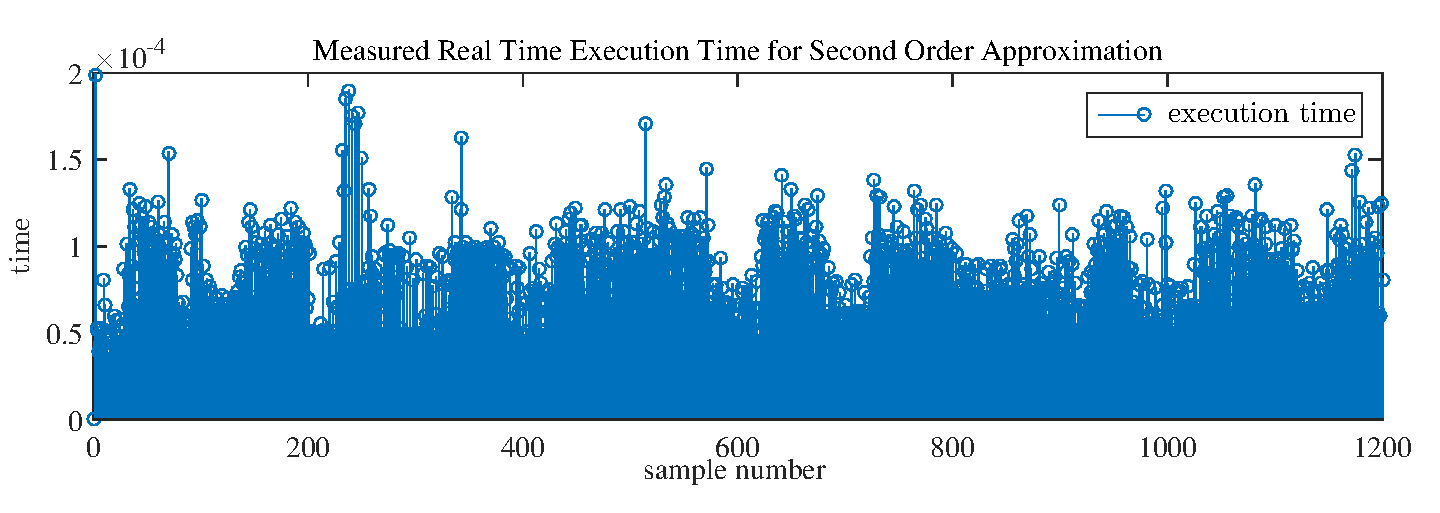
\includegraphics[scale=0.6]{execution_time_2_order.eps}
	\caption{Execution time for second order system approximation. It is seen that the controller never exceeds a computation time of 200\,$\mu$s.}
	\label{fig:exe_2}
\end{figure}



\vspace{-3mm}
\begin{figure}[H]
	\center
		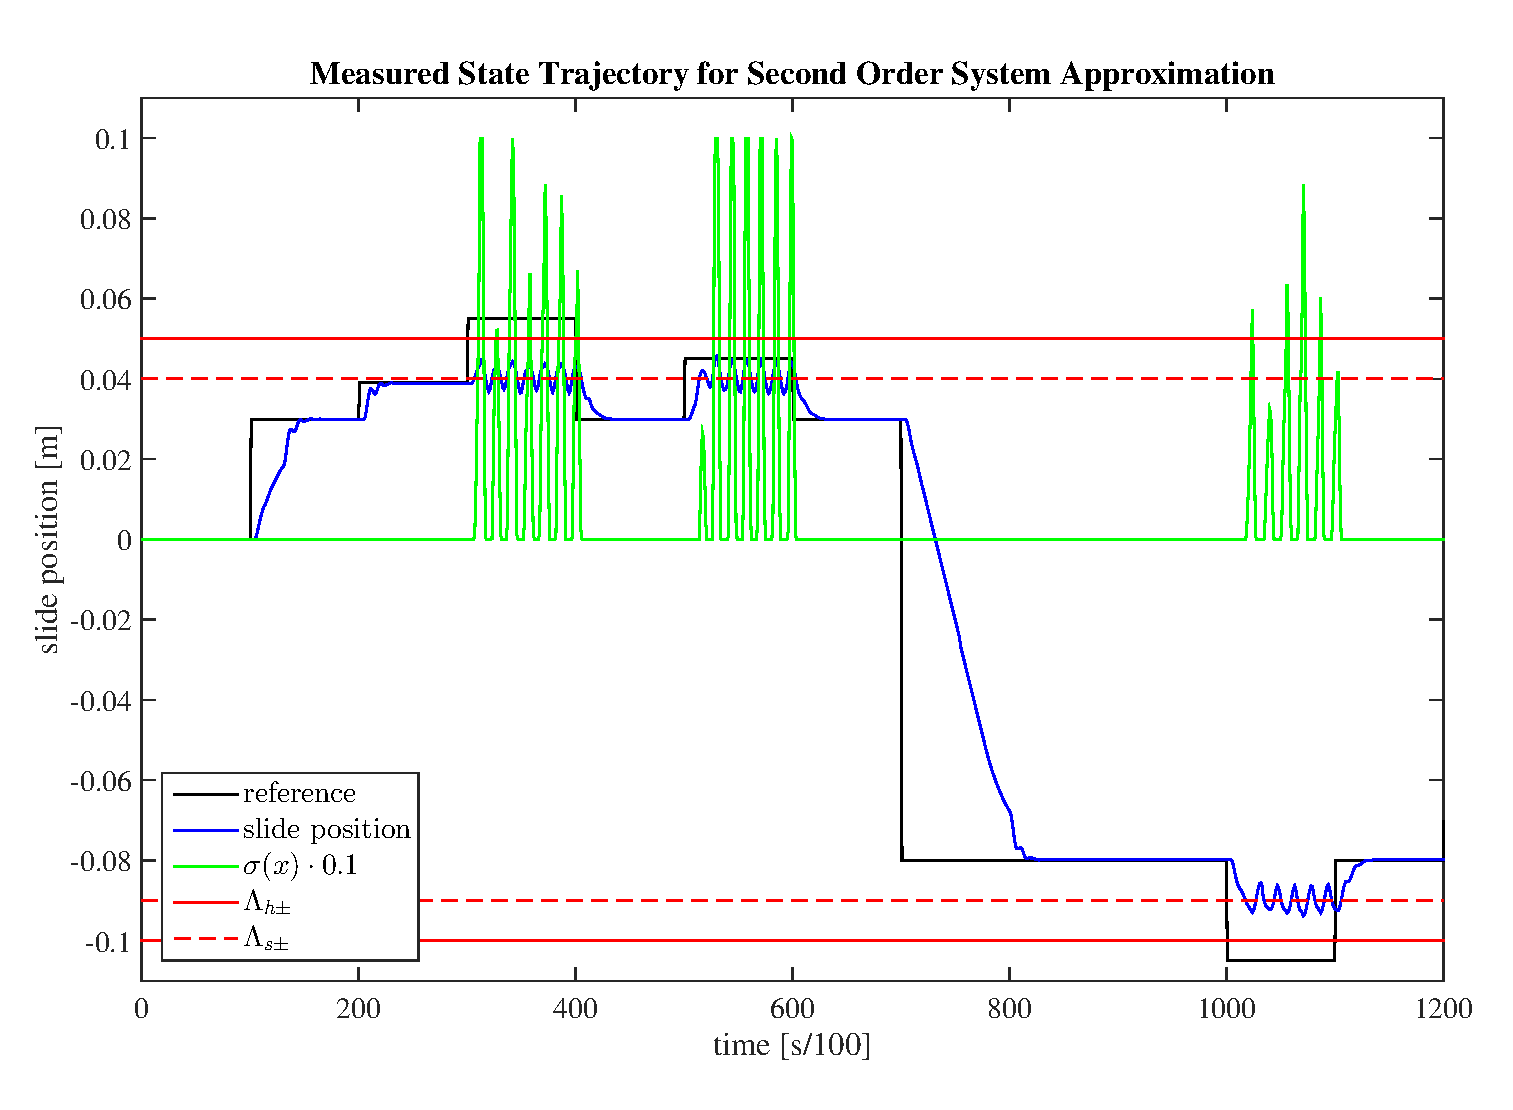
\includegraphics[scale=0.65]{meas_trajectory_2_order.eps}
	\caption{Measured position trajectory based on the second order approximation.}
    \label{fig:traj_meas_2}
\end{figure}
The measured state trajectory is plotted in \autoref{fig:traj_meas_2}, visualizing how the overshoot is eliminated, which was indeed the main purpose of the development of a controller based on a second order approximation. Also, note how it is possible to give setpoints close to the the set $\mathcal{T}$ and still avoid oscillations caused by $\sigma(\mathbf{x})\neq 0$. This is a big advantage when a doctor needs to operate close to an unsafe region. Finally, just as in \autoref{fig:traj_meas_1}, it is seen how $\sigma(\mathbf{x})$ allows $k_0(\mathbf{x})$ to force the position from reaching its setpoint when $x_\text{ref} \in \mathcal{X}_u$ but allows $x$ to cross $x_\text{ref}$ when $x_\text{ref} \in \mathcal{T}$, as is intended with $\sigma(\mathbf{x})$.

\begin{figure}[H]
	\center
		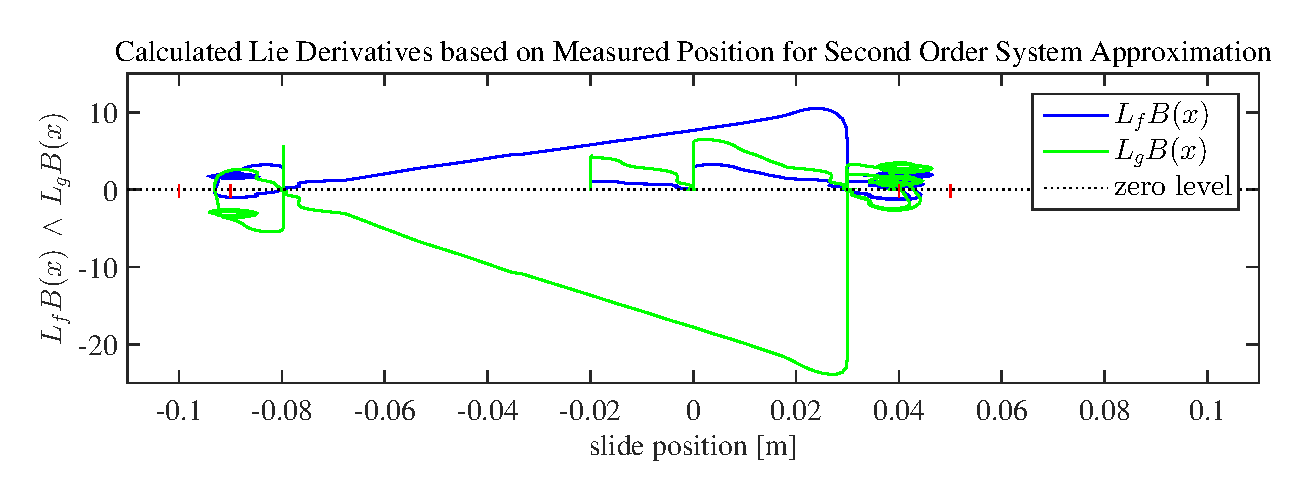
\includegraphics[scale=0.7]{meas_lie_2.eps}
	\caption{Calculated Lie derivatives based on measured position and estimated velocity for the second order system approximation. }
    \label{fig:meas_lie_2}
\end{figure}
The Lie derivatives are calculated based on the measured position and the estimated velocity. The result is seen in \autoref{fig:meas_lie_2} showing that the Lie derivatives  are quite different from the simulated derivatives in \autoref{fig:lie2}. This might be due to an imprecise state estimation.

\subsection{Conclusion for Slide Safety Controller}\label{subsec:conclusion-slide-safety}
In conclusion, this chapter verifies the usefulness of the theory presented in \autoref{chap:cbf} verifying that it complies with both simulation and real world implementation. It is seen how the trajectory is forced away from the unsafe region whenever setpoints are given in $\mathcal{X}_u$. The theory presented in \citep{bib:org_control} does indeed turn out to be very useful in practical implementations. It is worth noting that the construction of barrier certificates can be quite time consuming (especially when the state vector grows in order) and that the velocity causes some challenges when barrier certificates are constructed. For that reason, one may look in other directions when high order systems are considered.

The results from this chapter suggest some improvements in the current setup:
\begin{itemize}
\item Replace the TCP/IP communication channel with a \gls{udp} channel such that the topic \texttt{joint\_states} updates faster, i.e. preferably with 2\,kHz. This will  improve the precision and resolution and ultimately help save human lives.
\item Improve the transition region $\mathcal{T}$ such that precise setpoints can be given in this region. This could imply a purely non-linear controller in $\mathcal{T}$.
\item Improve the bump function $\sigma(\mathbf{x})$ for the second order system such that the braking distance is optimized.
\end{itemize}
The above considerations conclude this chapter.